\documentclass{article}
\usepackage{amsmath}
\usepackage{mathtools}
\usepackage{gensymb}
\usepackage[a4paper,inner=1.5cm,outer=1.5cm,top=2cm,bottom=0.5cm]{geometry} 
\usepackage{xcolor}                    
\usepackage{tikz}                           
\usepackage{multicol}
\usepackage{pgfplots}
\usetikzlibrary{calc}
\usetikzlibrary{intersections}
\usetikzlibrary{intersections,calc,angles,quotes}
\usetikzlibrary{shapes,arrows,positioning,decorations.pathreplacing,calc}
\usetikzlibrary{calc,angles,positioning,intersections,quotes,decorations.markings}
\usepackage{tkz-euclide}
\usetikzlibrary{backgrounds}
\usetikzlibrary{calc,through}
\usetikzlibrary{angles}
\usetikzlibrary{fadings}
\usetikzlibrary{shapes.geometric}
\usetikzlibrary{shapes.symbols}
\usepackage{draftwatermark}
\usepackage{mathptmx}

\SetWatermarkText{\textcolor{black!30}{Mathema Shukur}}
\SetWatermarkFontSize{2 cm}
\usepackage[utf8]{inputenc}
\usepackage{fontspec}

\setmainfont{[Kalpurush.ttf]}
\newfontface{\en}{[Arial.ttf]} %%this is optional, if you want to use a secondary font. Any english font is supported
\newlength\Radius
\setlength\Radius{4cm}
\begin{document} 
	\Large
	\textcolor{red}{Welcome To} 
	\\
	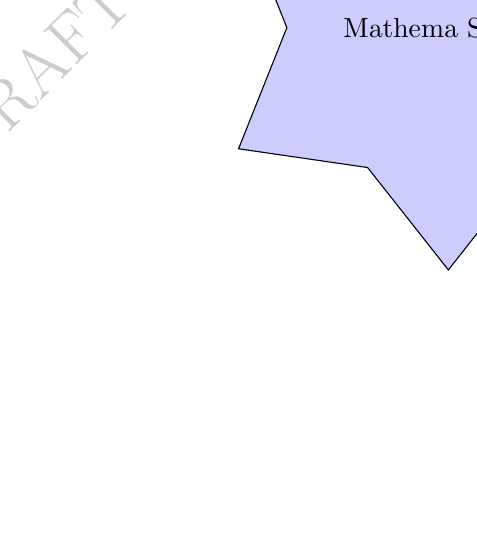
\begin{tikzpicture}
		\tikz \node [fill=blue!20,star,star points=6,draw] {Mathema Shukur };
	\end{tikzpicture}
	\\
	যাদের জন্যে প্রযোজ্যঃ  	\textcolor{magenta}{একাদশ ও দ্বাদশ শ্রেণীর শিক্ষার্থী} \\
	বিষয়ঃ \textcolor{magenta}{উচ্চতর গণিত ১ম পত্র} \\
	অধ্যায়ঃ \textcolor{magenta}{৩-সরলরেখা}\\ 
	Subtopicঃ  \textcolor{magenta}{ দুইটি সরলরেখার ছেদবিন্দু নির্ণয় }\\
	\\
	মনে করি, দুইটি সরলরেখার আদর্শ সমীকরণ \\ 
		\begin{align*}
			a_1x+b_1y+c_1&=0\\
			\\
			a_2x+b_2y+c_2&=0\\
		\end{align*}
		বজ্রগুণন সূত্রানুসারে\\ 		
		\begin{align*}
			\frac{x}{b_1c_2-b_2c_1}=\frac{y}{a_2c_1-a_1c_2}=\frac{1}{a_1b_2-a_2b_1}
		\end{align*}
	\begin{multicols}{2}
		\begin{align*}
		\frac{x}{b_1c_2-b_2c_1}&=\frac{1}{a_1b_2-a_2b_1}\\
		\\
		x&=\frac{b_1c_2-b_2c_1}{a_1b_2-a_2b_1}
	\end{align*}
	\\
	\begin{align*}
		\frac{y}{a_2c_1-a_1c_2}&=\frac{1}{a_1b_2-a_2b_1}\\
		\\
		y&=\frac{a_2c_1-a_1c_2}{a_1b_2-a_2b_1}
	\end{align*}
	\end{multicols}
ছেদবিন্দুর স্থানাঙ্ক $\left(\frac{b_1c_2-b_2c_1}{a_1b_2-a_2b_1},\frac{a_2c_1-a_1c_2}{a_1b_2-a_2b_1}\right)$\\ 
\\
যদি $a_1b_2-a_2b_1=0$ হয়  তবে রেখা দুইটি পরস্পর সমান্তরাল হবে। এক্ষেত্রে ছেদবিন্দু অসীমে পাওয়া যাবে অর্থাৎ ছেদবিন্দু নাই।রেল লাইন জোড়াকে উদাহরণ হিসাবে বিবেচনা করা যায়। \\
\\
ঢাকা বোর্ড-২০১৬\\ 
$2x-y-1=0$ এবং $3x-4y+6=0$ রেখা দুইটির ছেদবিন্দু নির্ণয় কর \\
\\
$2x-y-1=0$,\quad $a_1=2,\quad b_1=-1,\quad c_1=-1$\\
\\
$3x-4y+6=0$ ,\quad $a_2=3,\quad b_2=-4,\quad c_2=6$\\
\\
\begin{align*}
&\left(\frac{b_1c_2-b_2c_1}{a_1b_2-a_2b_1},\frac{a_2c_1-a_1c_2}{a_1b_2-a_2b_1}\right)\\
\\
&\left(\frac{(-1)(6)-(-4)(-1)}{(2)(-4)-(3)(-1)},\frac{(3)(-1)-(2)(6)}{(2)(-4)-(3)(-1)}\right)\\
\\
&\left(\frac{(-1)(6)-(-4)(-1)}{(2)(-4)-(3)(-1)},\frac{(3)(-1)-(2)(6)}{(2)(-4)-(3)(-1)}\right)\\
\\
&\left(\frac{-6-4}{-8+3},\frac{-3-12}{-8+3}\right)\\
\\
&\left(\frac{-10}{-5},\frac{-15}{-5}\right)\\
\\
&\left(2,3\right)
\end{align*}
\\
	\begin{tikzpicture}[transform shape,scale=1]
	\draw [-latex,thick](-6,0) -- (6,0) node[right] {$x$} coordinate(x axis);
	\draw [-latex,thick](0,-3) -- (0,7) node[above] {$y$} coordinate(y axis);
	\fill[black] (0,0) circle (1 mm);
	\node at (0.3,-0.3) {$\textcolor{purple}{O}$};	
	\node at (6,4.5) {$\textcolor{blue}{3x-4y+6=0}$};	
	\node at (1.8,5.5) {$\textcolor{green}{2x-y-1=0}$};	
		\node at (3,3) {$\textcolor{red}{(2,3)}$};	
	\draw[very thick,green] (-1,-3)--(3,5);	
	\draw[very thick,blue] (-6,-3)--(6,6);	
	\fill[red] (2,3) circle (1 mm);
\end{tikzpicture}
\\
(KUET-2014-2015)\\ 
$3x+2y=9$ এবং $2x+3y=11$ রেখা দুইটির ছেদবিন্দু নির্ণয় কর \\
\\
সমীকরণদ্বয় যেকোনো পদ্ধতিতে সমাধান করলেই ছেদবিন্দুর স্থানাঙ্ক পাওয়া যাবে\\ 
\\
$3x+2y=9$,$\Rightarrow$\quad $6x+4y=18$\\
\\
$2x+3y=11$,$\Rightarrow$ \quad $6x+9y=33$\\
\\
$(6x-6x)+(9y-4y)=33-18$\\
\\
$5y=15$,$\Rightarrow$ \quad $y=3$\\
\\
\begin{align*}
3x+2y&=9\\
\\
3x+2(3)&=9\\
\\
3x+6&=9\\
\\
3x&=3\\
\\
x&=1
\end{align*}
\\
ছেদবিন্দুর স্থানাঙ্ক $(1,3)$
\\
	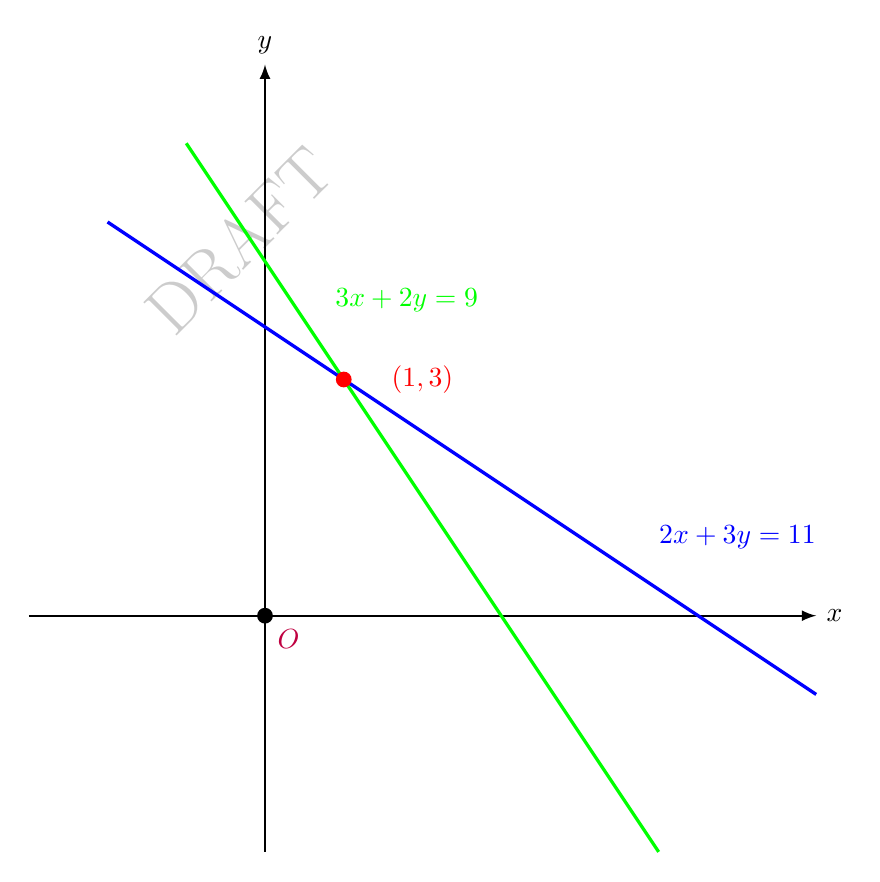
\begin{tikzpicture}[transform shape,scale=1]
	\draw [-latex,thick](-3,0) -- (7,0) node[right] {$x$} coordinate(x axis);
	\draw [-latex,thick](0,-3) -- (0,7) node[above] {$y$} coordinate(y axis);
	\fill[black] (0,0) circle (1 mm);
	\node at (0.3,-0.3) {$\textcolor{purple}{O}$};	
	\node at (6,1) {$\textcolor{blue}{2x+3y=11}$};	
	\node at (1.8,4) {$\textcolor{green}{3x+2y=9}$};	
	\draw[very thick,green] (-1,6)--(5,-3);	
	\draw[very thick,blue] (-2,5)--(7,-1);	
	\fill[red] (1,3) circle (1 mm);
		\node at (2,3) {$\textcolor{red}{(1,3)}$};	
\end{tikzpicture}
\end{document}